\documentclass[../main]{subfiles}
\begin{document}




\setcounter{chapter}{6}
\chapter{Fuerza electro motriz inducida}
\img{images/06/feminducida}{Fem inducida en un conductor que se mueve perpendicular a un campo magnético}

\section{Conductor rectilíneo que se mueve en campo magnético}


 \begin{center}
 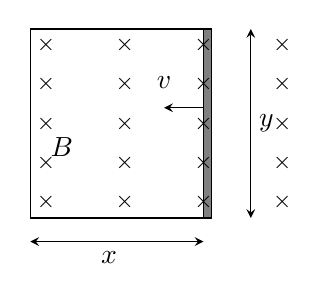
\begin{tikzpicture}
 \draw [stealth-stealth](0.6,-0.2) -- (0.6,2.2);
 \draw [stealth-stealth](-2.2,-0.5)-- (0,-0.5);
 \draw [](-2.2,-0.2) rectangle (0,2.2);
 \node at (0.8,1) {$y$};
 \node at (-1.2,-0.7) {$x$};
 \node at (-1.8,0.7) {$B$};
 
 \draw [fill=gray](0,-0.2) rectangle (0.1,2.2);
 \draw [-stealth] (0,1.2) -- (-0.5,1.2)  node[label={$v$}]{};
 \foreach \y in {0,1,2,...,4}{
    \foreach \x in {-4,-2,...,2}{
    \node at (\x/2,\y/2) {\footnotesize $\times$};
    }
}
 \end{tikzpicture}
 \end{center}

Suponiendo que tenemos un conductor de longitu $y$ que se mueve a velocidad $v=\frac{\Delta x}{\Delta t}$ haciendo contacto en sus extremos sobre una vía de dos conductores perpendiculares a este de longitud $x$ unidas en su extremo que forman todo en su conjunto una espira de superficie $S=x \times y$, y es cortado perpendicularmente a la superficie por una inducción $B$. Según la ley de Faraday-Lenz tenemos que: 
\begin{equation}
    E_m= -N \dfrac{ \Delta \Phi}{\Delta t}
\end{equation}
Como se trata de una espira $N=1$, la variación de superficie 
$\Delta S =\Delta x \times y$ y como $\Delta \Phi=B \times \Delta S $ podemos reemplazar y nos queda.
\begin{equation}
    E_m= -1 \dfrac{ B \times \Delta S}{\Delta t}
\end{equation}
Como sabemos que $\Delta S =\Delta x \times y$ reemplazamos
\begin{equation}
    E_m= - \dfrac{ B \times \Delta x \times y}{\Delta t}
\end{equation}
El signo negativo lo eliminamos por que la dirección la determinaremos con la regla de la mano izquierda. Y además sabemos que $v=\frac{\Delta x}{\Delta t}$ podemos reemplazar en la formula.

\begin{equation}
    E_m=   B \times v \times y
\end{equation}

Ademas sabemos que $y$ es la longitud del conductor, podemos usar $l$ para recordar que se trata de la longitud. Reemplazamos:
\begin{equation}
    E_m=   B \times v \times l
\end{equation}







\info{Fuerza electro motriz inducida $E$ en un conductor que se mueve perpendicular a un campo magnético}{
La fuerza electromotriz $E$ (F.E.M) inducida en un conductor es igual al producto de la inducción magnética $B$, la longitud del conductor dentro del campo magnético $l$, y la velocidad del conductor $v$.

\begin{equation*}
    E = B \times l \times v
\end{equation*}
siendo:

$E$: Fuerza electromotriz inducida en volts $[V]$.

$B$: Inducción del campo magnético en teslas $[T]$.

$V$: Velocidad con que se mueve el conductor $[m/s]$.

$l$: Longitud del conductor en metros $[m]$.
}
\actividad{Resolver los siguientes problemas.}
\begin{enumerate}
    \item Un conductor que se desplaza con una velocidad $v=3\frac{m}{s}$ perpendicular a un campo magnético de inducción $B=1T$, sabiendo que la longitud es $l=20cm$. Calcular la \textbf{fuerza electro motriz} $F.E.M$ inducida en el conductor.

    \item Un conductor rectilíneo se desplaza perpendicularmente a la dirección de un campo magnético de inducción $B=18000Gauss$, con una velocidad de $v=2\frac{m}{s}$. Calcular la \textbf{longitud del conductor} si está dentro del campo magnético si que induce en el una F.E.M de $E=14V$.
    
    \item Un conductor que se desplaza con una velocidad $v=100\frac{Km}{h}$  en un campo magnético de inducción $B=300Gs$, sabiendo que la longitud es $l=200mm$. Calcular la el \textbf{voltaje} ($F.E.M$) inducido.

    \item Un conductor que se desplaza con una velocidad $v=10\frac{m}{s}$  en un campo magnético de inducción $B=2T$, sabiendo que la longitud es $l=10cm$. Calcular la \textbf{corriente} que circula por el conductor si se conecta a una resistencia de $R_L=10\Omega$.

    
    \item Calcular la \textbf{velocidad} que debe llevar un alambre de longitud $l=20cm$ que se desplaza en un campo de inducción $B=1.4T$, para que la \textbf{F.E.M. inducida} sea de $E=2V$.

    \item Un conductor de longitud $l=30cm$ se mueve perpendicularmente al campo con una velocidad de $v=4\frac{m}{s}$. Calcular el valor de la \textbf{inducción $B$} si la F.E.M. inducida es de $E_m=18V$.
    
    \item Si un conductor tiene $l=0,5m$ de longitud dentro de un campo magnético de inducción $B=2T$, se desplaza perpendicular a la líneas de fuerza con una velocidad de $v=4\frac{m}{s}$. Calcular la \textbf{F.E.M} inducida $E$, la intensidad de la corriente $I$ conectando una resistencia de $R=12\Omega$.
    
    \item Un conductor metálico de longitud $l=0.8 m$ se desplaza a través de un campo magnético uniforme con una velocidad de $v=3 m/s$. La fuerza electromotriz (fem) inducida en el conductor es de $E_m=0.6 V$. Calcula la \textbf{inducción} ($B$).

    \item Un conductor metálico se desplaza a través de un campo magnético uniforme con una velocidad de $v=4 m/s$. La fuerza electromotriz (fem) inducida en el conductor es de $F.E.M=1,2 V$. Si la intensidad del campo magnético es de $B=0,2 T$, ¿cuál es la \textbf{longitud} del conductor dentro del campo magnético en centímetros?

    \item Un conductor metálico se desplaza a través de un campo magnético uniforme con una inducción de $B=3000Gs$. La fuerza electromotriz (fem) inducida en el conductor es de $V=0,9 V$. Si la longitud del conductor dentro del campo magnético es de 150 centímetros, ¿cuál es la \textbf{velocidad} del conductor en $Km/h$?

    \item Un alambre conductor de longitud \( l = 0.6 \, \text{m} \) se mueve perpendicularmente a través de un campo magnético uniforme con una velocidad de \( v = 2 \, \text{m/s} \). Si la inducción magnética es \( B = 0.4 \, \text{T} \), ¿cuál es la \textbf{fuerza electromotriz (F.E.M)} inducida en el alambre?
    
    \item Un objeto conductor se desplaza a través de un campo magnético uniforme con una velocidad de \( v = 5 \, \text{m/s} \). Si la densidad de flujo magnético es \( B = 0.2 \, \text{T} \) y la fem inducida es de \( V = 1.5 \, \text{V} \), ¿Cuál es la \textbf{longitud} del conductor dentro del campo magnético?
    
    \item Una barra metálica de longitud \( l = 0.8 \, \text{m} \) se desplaza a través de un campo magnético uniforme con una inducción magnética de \( B = 0.5 \, \text{T} \). Si la fem inducida es de \( V = 1.2 \, \text{V} \), ¿A qué \textbf{velocidad} se mueve la barra?
    
    \item Un alambre conductor de longitud \( l = 0.7 \, \text{m} \) se desplaza paralelamente a través de un campo magnético uniforme con una inducción magnética de \( B = 0.6 \, \text{T} \). Si la velocidad del conductor es \( v = 3 \, \text{m/s} \), ¿Cuál es la \textbf{fuerza electromotriz} inducida en el alambre?


    \item Un cable conductor se desplaza a través de un campo magnético uniforme con una inducción magnética de \( B = 0.3 \, \text{T} \). Si la fem inducida es de \( V = 0.7 \, \text{V} \) y la longitud del conductor dentro del campo magnético es de \( l = 0.4 \, \text{m} \), ¿Cuál es la \textbf{velocidad} del conductor?
    
    \item Un conductor se desplaza a través de un campo magnético uniforme con una velocidad de \( v = 4 \, \text{m/s} \). Si la fem inducida es de \( V = 1.8 \, \text{V} \) y la inducción magnética es \( B = 0.4 \, \text{T} \), ¿Cuál es la \textbf{longitud del conductor} dentro del campo magnético?    
\end{enumerate}
\end{document}